\subsection{\textcolor{Salmon}{Ergebnisse Usability Test}}
\textcolor{blue}{\textit{einleitende Worte}}\\

\noindent
\underline{Fehlerbetrachtung}\\
- Fehlende Daten aus Gründen xy\\

\noindent
\underline{Genauigkeit-Zeit-Vergleich}\\

\noindent
\underline{s. \autoref{tab:usability_test:mittelwerte}}\\
- Differenz berechnen, Fehlerquote als Wert\\
-> Berechnung Fehlerquote in Tabelle im Anhang \autoref{fig:Usability-Test:Excel_Berechnungen}\\
- grafisch dargestellt in \autoref{fig:usability_test:genauigkeit-zeit_alt-neu} \&\& \autoref{fig:usability_test:genauigkeit-zeit_alle-richtige}

%\subsection{Genauigkeit-Zeit}
\begin{figure}[H]
    \centering
    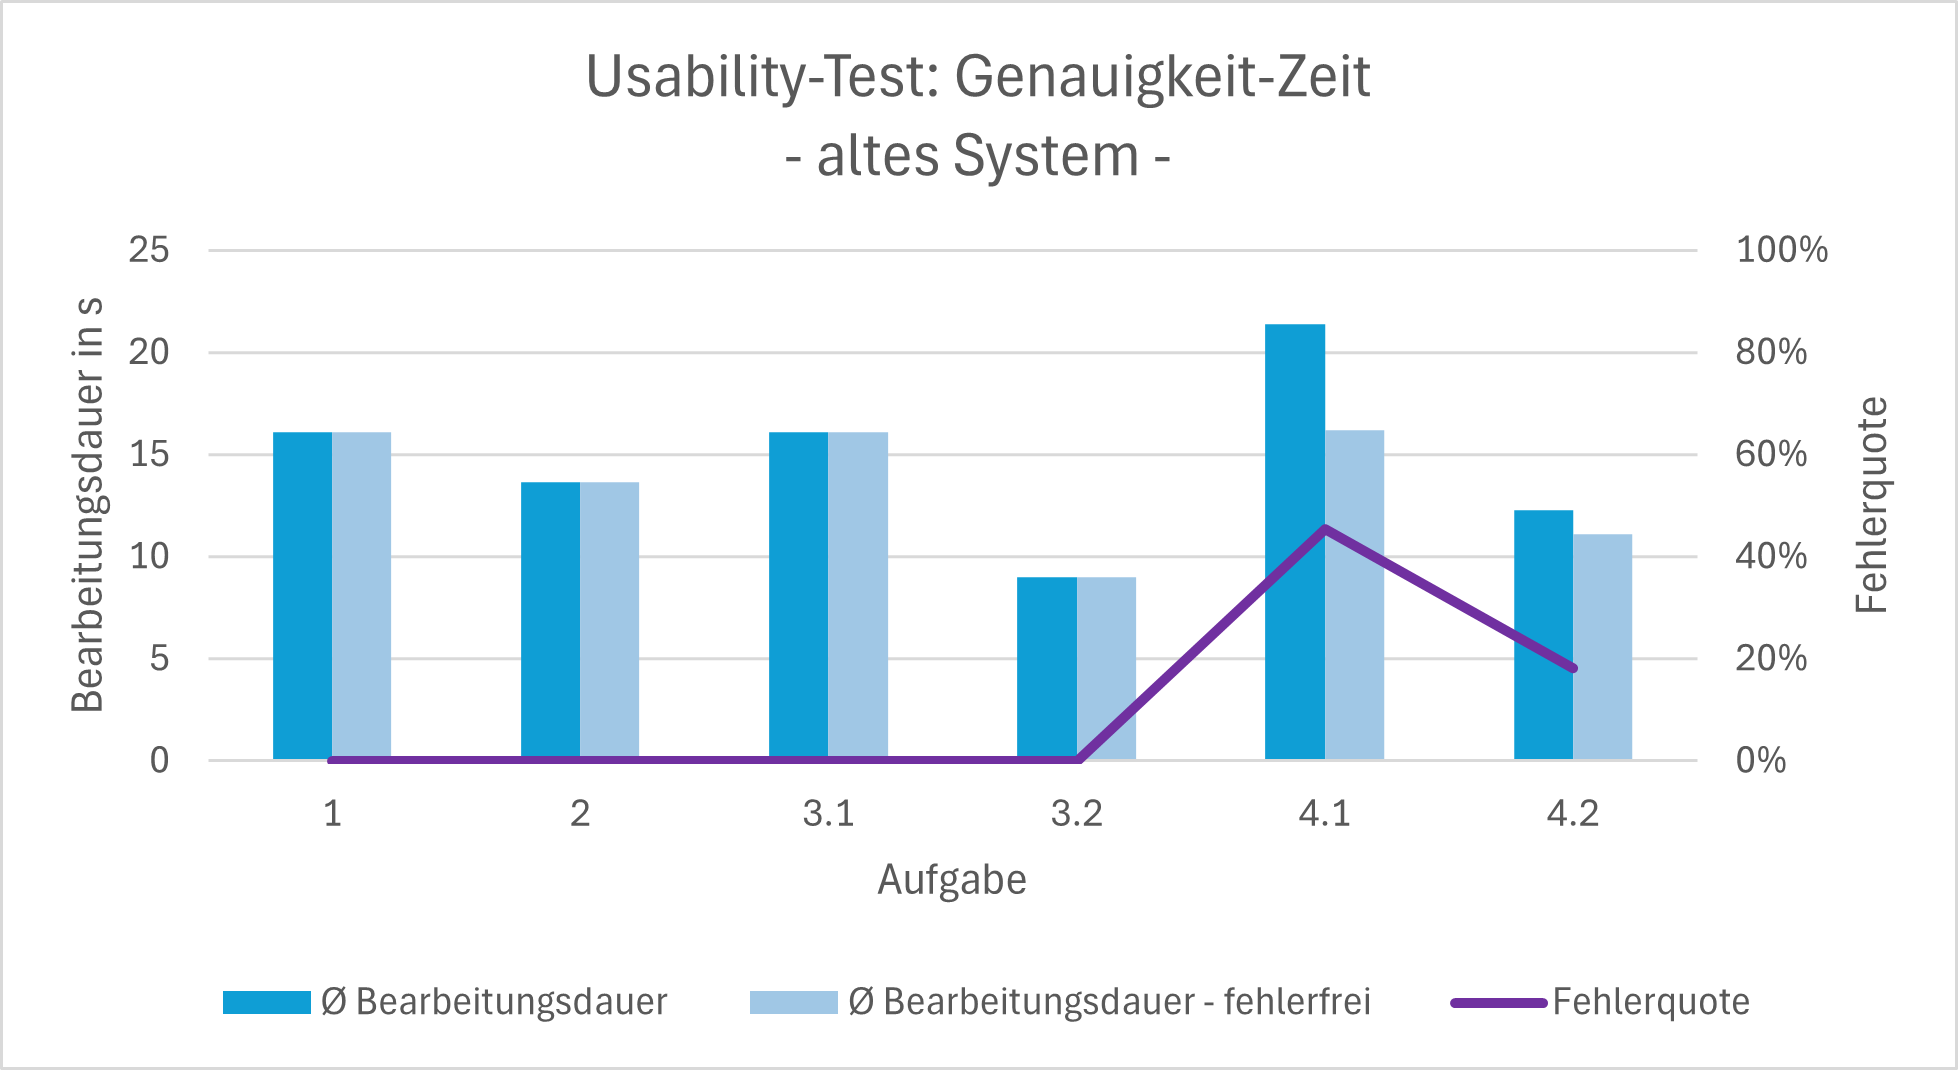
\includegraphics[width=0.8\linewidth]{Diagramme/usability_genauigkeit-zeit_alt.png}
    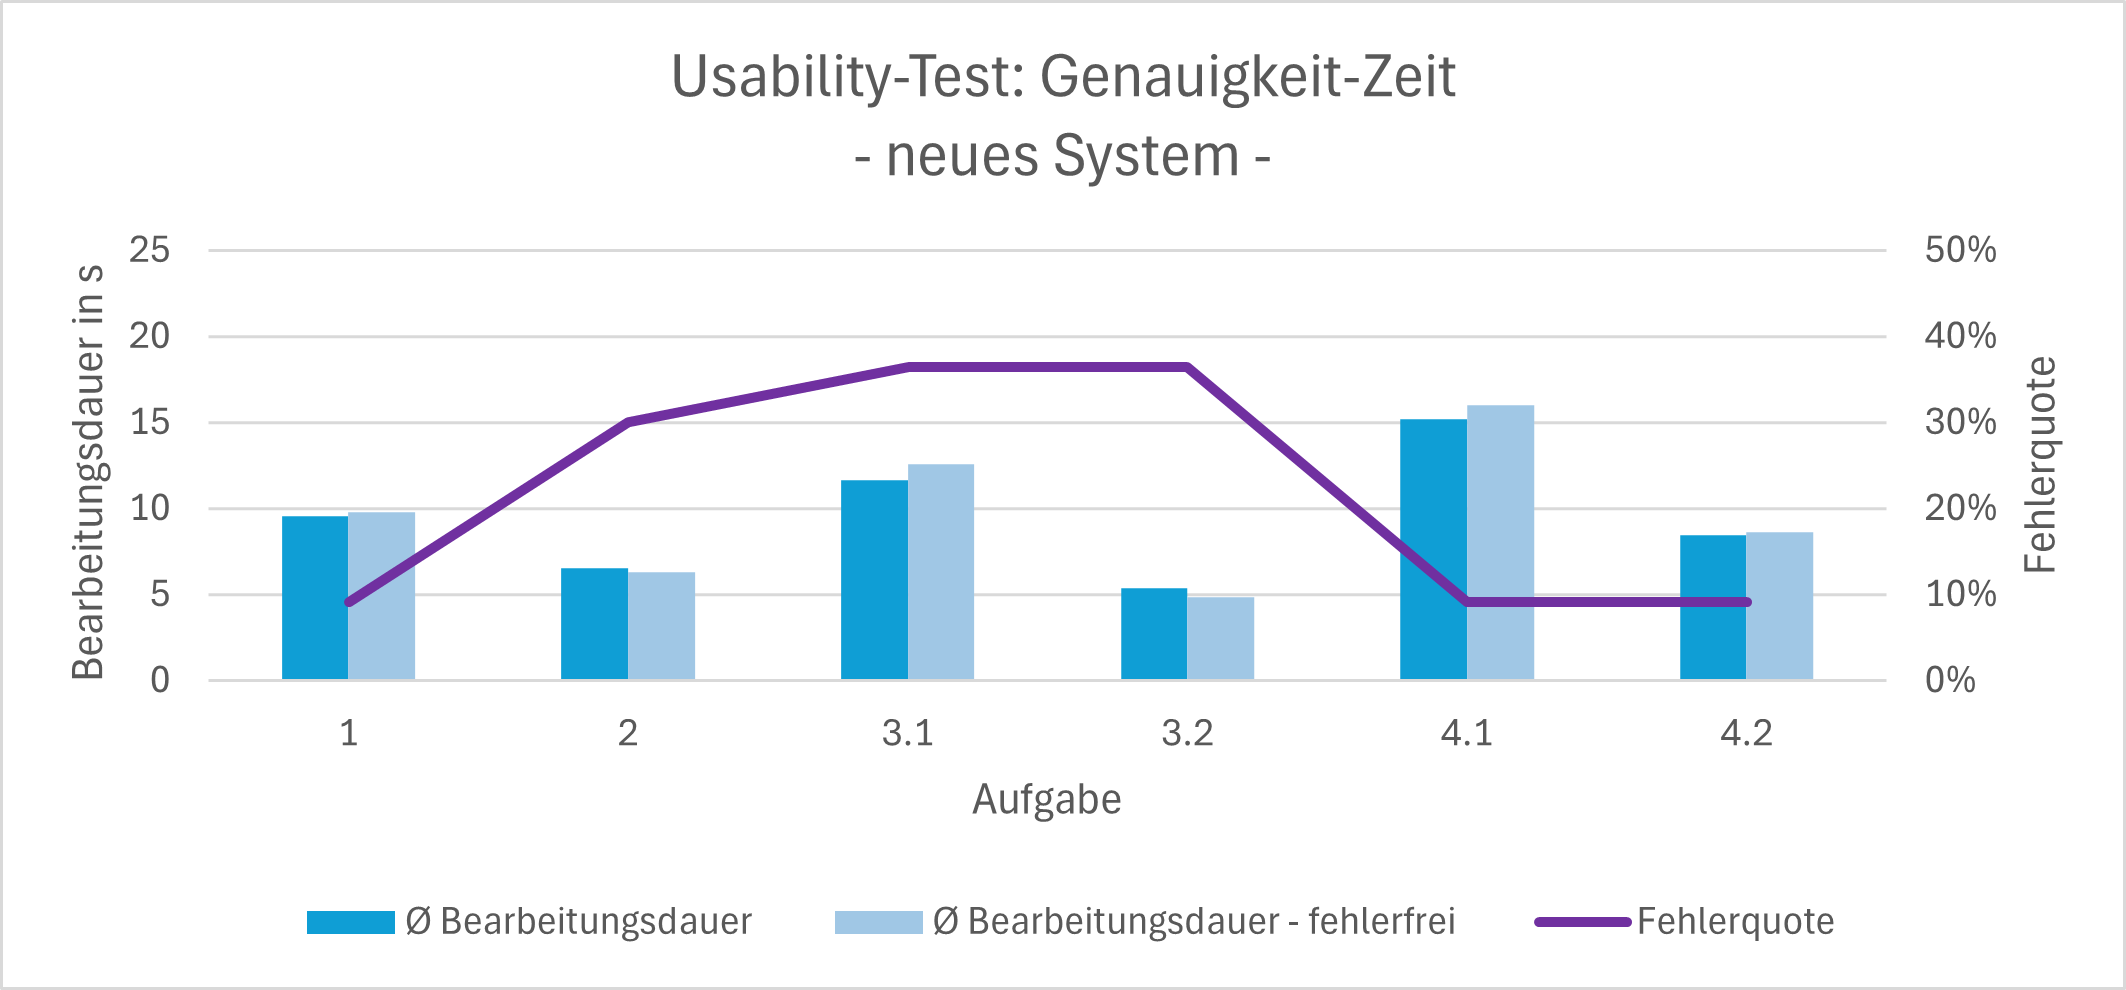
\includegraphics[width=0.8\linewidth]{Diagramme/usability_genauigkeit-zeit_neu.png}
    \caption{Usability-Test: Vergleich Genauigkeit-Zeit im alten und neuen System}
    \label{fig:usability_test:genauigkeit-zeit_alt-neu}
\end{figure}

\noindent
\underline{s. \autoref{fig:usability_test:genauigkeit-zeit_alt-neu}}\\
- alt: Leute mit Fehlern waren langsamer\\
- neu: Leute ohne Fehler waren minimal langsamer, kein signifikanter Unterschied\\
- neu: höhere Fehlerquote, dafür auch x\% schneller (Bsp. Frage 1: 15s auf 10s)\\
-> bei Diskussion darauf eingehen, woher die höhere Fehlerquote kommt

\begin{figure}[H]
    \centering
    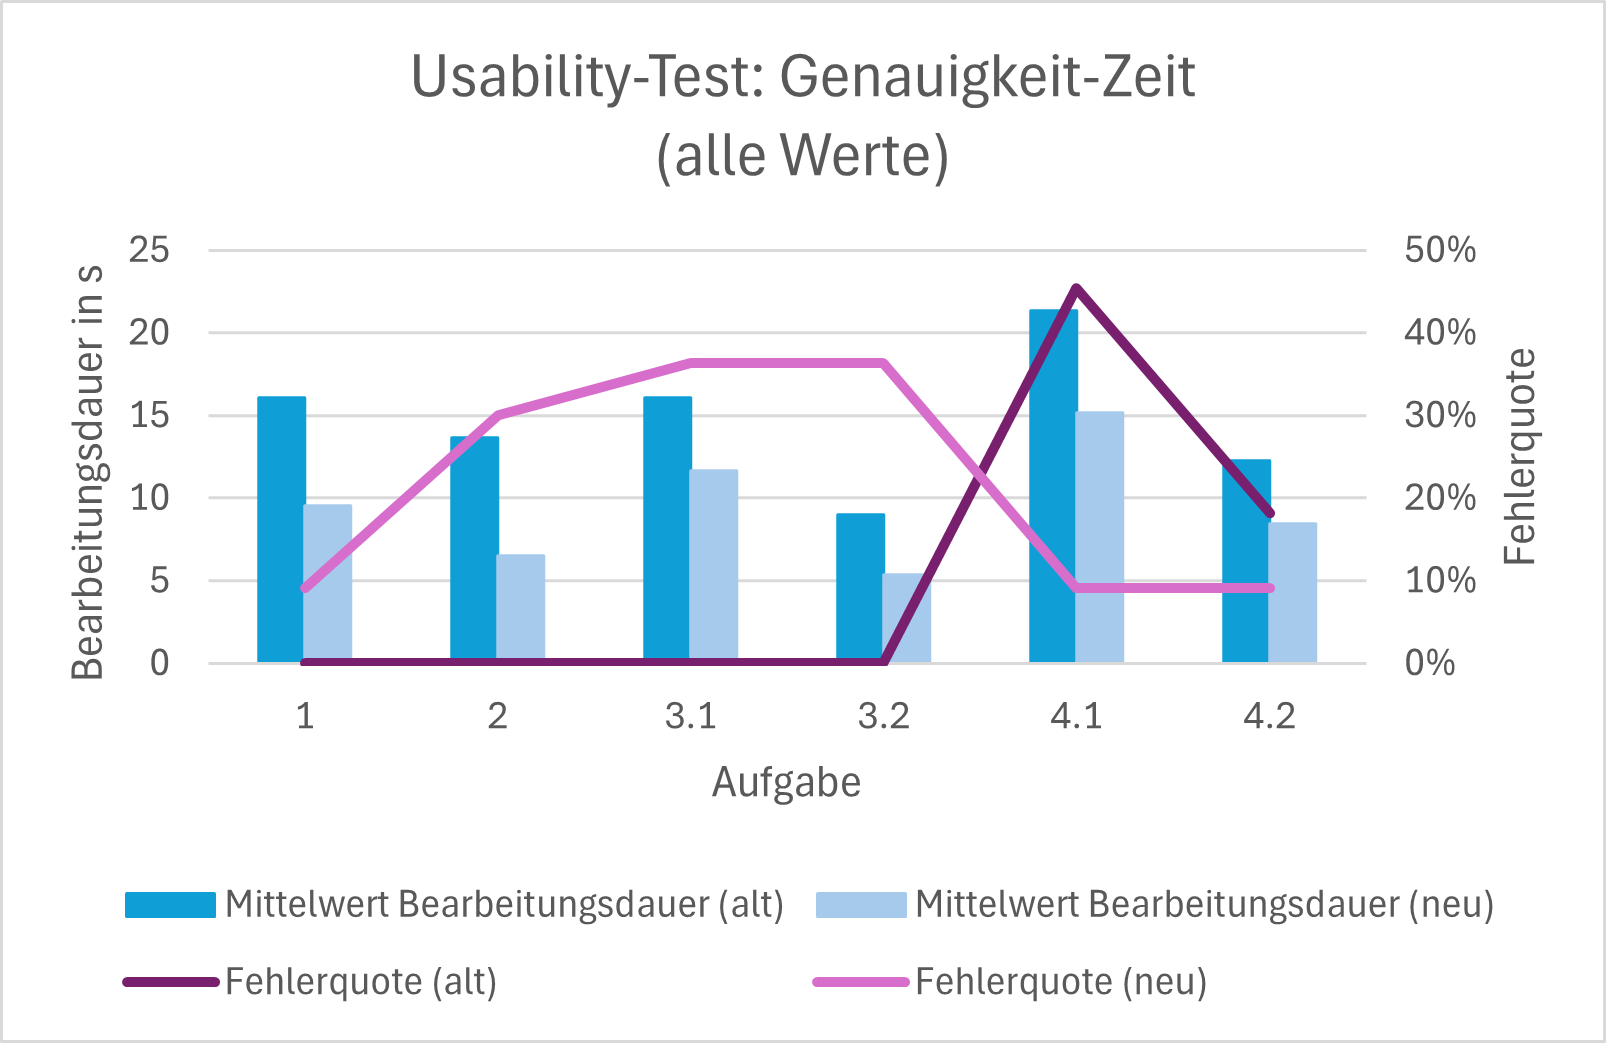
\includegraphics[width=0.8\linewidth]{Diagramme/usability_genauigkeit-zeit_alle.png}
    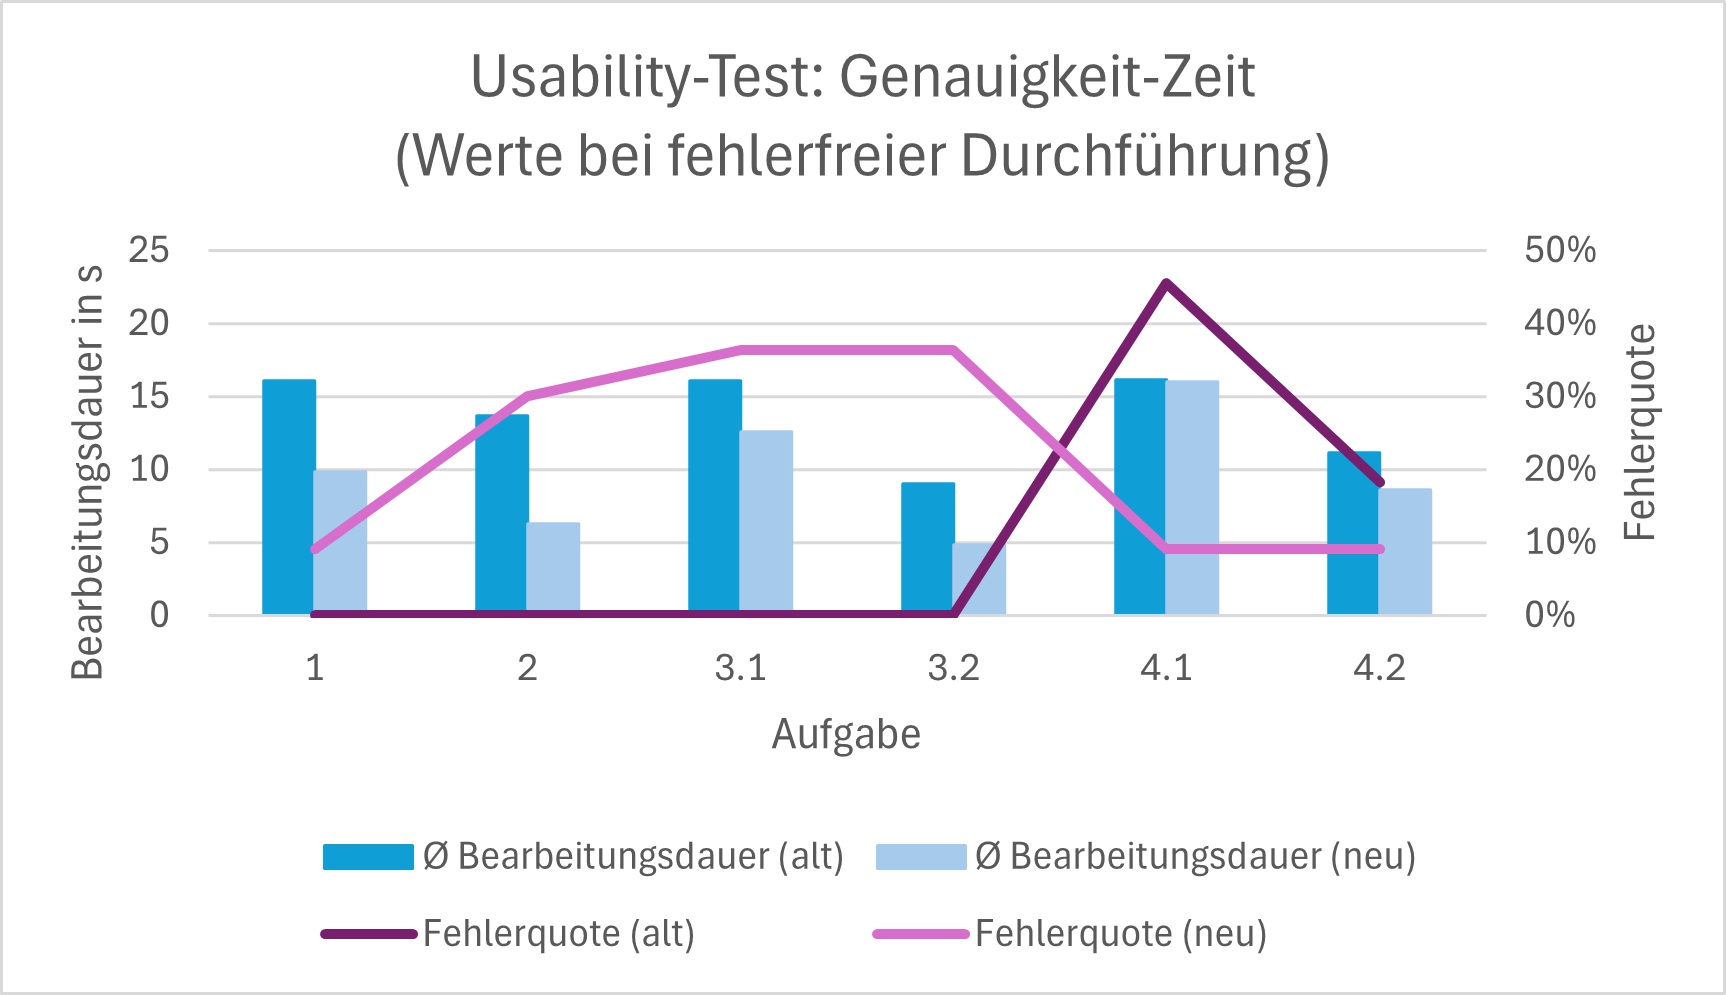
\includegraphics[width=0.8\linewidth]{Diagramme/usability_genauigkeit-zeit_richtige.png}
    \caption{Usability-Test: Zeitvergleich von allen Werten und nur richtigen Antworten - im Verhältnis zur Fehlerquote}
    \label{fig:usability_test:genauigkeit-zeit_alle-richtige}
\end{figure}

\noindent
\underline{s. \autoref{fig:usability_test:genauigkeit-zeit_alle-richtige}}\\
- neu ist in jeder Aufgabe ersichtlich schneller\\
-> Frage nach signifikanz\\
- Fehlerquote nicht überall eindeutig\\

\noindent
\underline{Statistische Auswertung der Signifikanz}\\
\label{Bsp:ttest}
- t-Test Beispielrechnung (einseitig, gepaart)\\
-> erster t-Test zum Verständnis\\
-> erst Normalverteiltes Ergebnis\cite{normalverteilung_rechner}\\
-> die Beispielrechnung gehört in den Text \cite{Statistik:Boertz:2010} \cite{Statistik:Sedlmeier:2024}\\
- Tabelle mit t-Test-Ergebnissen \autoref{tab:usability_test:Differenz+ttest}\\
-> Rest: verweisen auf Ergebnisse aus Excel: $=TTEST(Matrix_{alt}, Matrix_{neu},1,1)$ (s. \autoref{fig:Usability-Test:Excel_Berechnungen})

\noindent
- Zeiten sind im neuen Systen in Aufgaben 1+2 signifikant besser als im alten System\\
-> beim Rest nur besser, nicht signifikant\\
- endgültiger Zeitvergleich, s. Zusammenfassung \autoref{fig:usability_test:genauigkeit-zeit_mittel}

\begin{figure}[H]
    \centering
    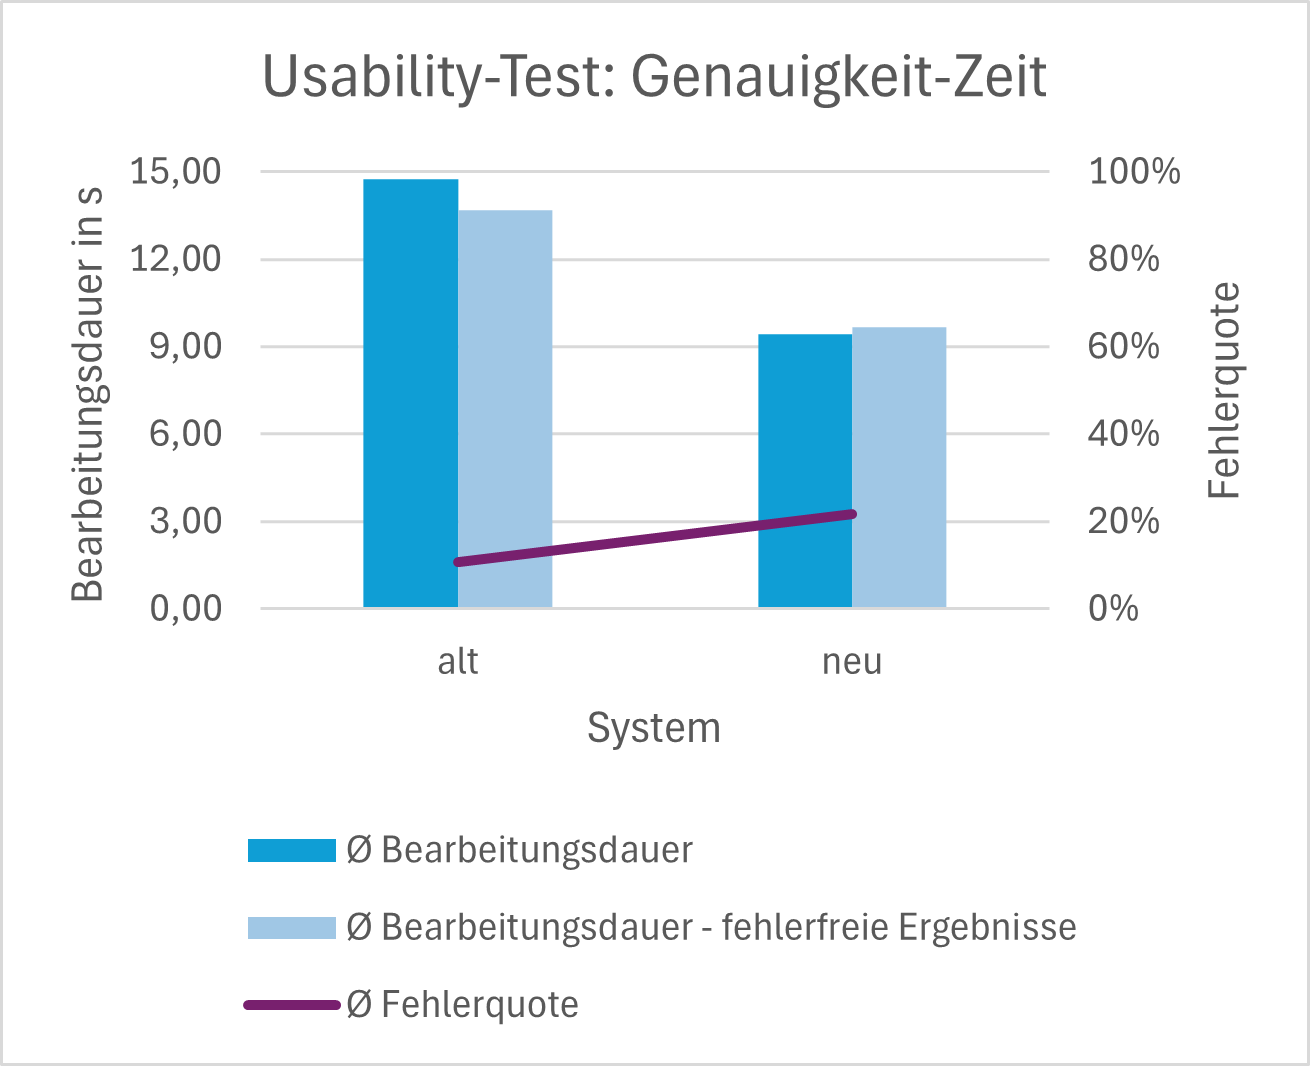
\includegraphics[width=0.8\linewidth]{Diagramme/usability_genauigkeit-zeit_mittel.png}
    \caption{Usability-Test: Vergleich der mittleren Bearbeitungsdauer - im Verhältnis zur Fehlerquote \textcolor{red}{Wo kommen die Daten her?}}
    \label{fig:usability_test:genauigkeit-zeit_mittel}
\end{figure}

\noindent
=> \ref{fig:usability_test:genauigkeit-zeit_mittel} erst in Diskussionskapitel(?)\\
- neu ist im Mittel schneller\\
- aber auch Fehlerquote bei neu im MIttel höher\\
- schöne Zusammenfassung (man kann auch darauf vorspringen)

